\section{Software Development Life Cycle}\label{sec:se-sdlc}
An implementation of the SDLC consists of two major components. First, the process is broken down into several smaller phases. Depending on the nature of the software, it is possible to omit steps or add more steps. I have compiled a simple yet generic approach from multiple sources \cite{2010govardhan} \cite{7106435}, to which most software projects adhere. This approach consists of five phases.
\begin{enumerate}
	\bolditem{Requirements phase} This is the initial phase of the development process. During this phase, the developer gets acquainted with the project and compiles a list of the desired functionalities \cite{7106435}. Using this information, the developer eventually decides on the required hardware specifications and possible external software which will need to be acquired.
	
	\bolditem{Design phase} After the developer has gained sufficient knowledge about the project requirements, they can use this information to draw an architectural design of the application. This design consists of multiple documents, including user stories and UML-diagrams.
	
	\bolditem{Implementation phase} During this phase, the developer will write code according to the specifications defined in the architectural designs.
	
	\bolditem{Testing phase} This is the most important phase. During this phase, the implementation is tested to identify potential bugs before the application is used by other users.
	
	\bolditem{Operational phase} In the final phase, the project is fully completed and it is integrated in the existing business environment.
\end{enumerate}

\noindent Subsequently, a model is chosen to define how to transition from one phase into another phase. A manifold of models exist \cite{2010govardhan}, each having advantages and disadvantages, but I will consider the basic yet most widely used model, which is the Waterfall model by Benington \cite{united1956symposium}. The initial Waterfall model required every phase to be executed sequentially and in order, cascading. However, this imposes several issues, the most prevalent being the inability to revise design decisions taken in the second phase, when performing the actual implementation in the third phase. To mitigate this, an improved version of the Waterfall model was proposed by Royce \cite{Royce:1987:MDL:41765.41801}. This version allows a phase to transition to a previous phase, as illustrated in \autoref{fig:waterfall-royce}.

\begin{figure}[htbp!]
	\centering
	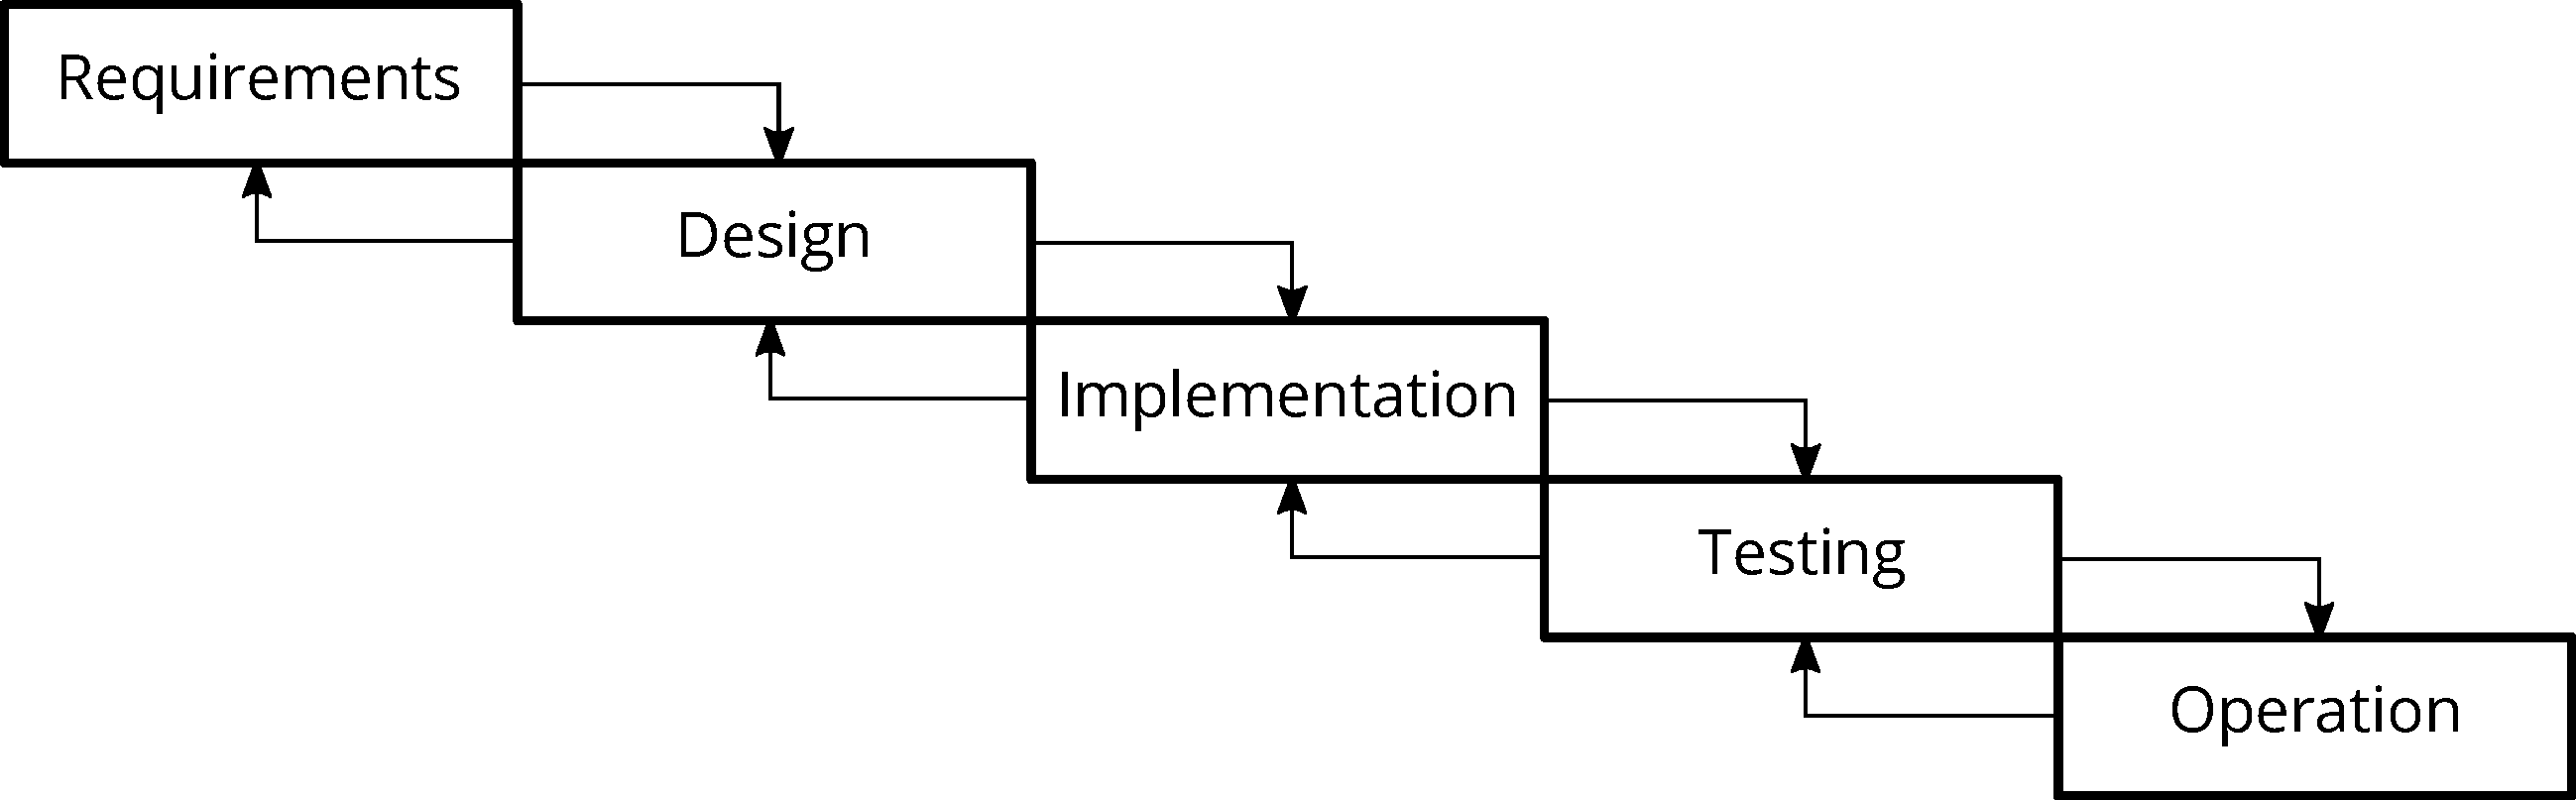
\includegraphics[width=\textwidth]{assets/sdlc.pdf}
	\caption{Improved Waterfall model by Royce}
	\label{fig:waterfall-royce}
\end{figure}

\noindent In this thesis I will solely focus on the implementation and testing phase, as these are the most time-consuming phases of the entire process. The modification to the Waterfall model by Royce is particularly useful when applied to these two phases, in the context of \emph{software regressions}. A regression \cite{10.1007/978-3-540-77966-7_18} is a feature that was previously working correctly, but is now malfunctioning. This behaviour can have external causes, such as a change in the system clock because of daylight saving time, but can also be the result of a change to another, seemingly unrelated part of the application code \cite{6588537}.\\

\noindent Software regressions and other functional bugs can ultimately incur disastrous effects, such as severe financial loss or damage to the reputation of the software company. The most famous example in history is without any doubt the explosion of the Ariane 5-rocket, which was caused by an integer overflow \cite{581900}. In order to reduce the risk of bugs, malfunctioning components should be detected as soon as possible to proactively defend against potential failures. Because of this reason, the testing phase is to be considered as the most important phase of the entire development process and an application should therefore include sufficient tests. The collection of all tests included in an application, or a smaller chosen subset of certain tests, is referred to as the \emph{test suite}. Tests can be classified in multiple categories, this thesis will consider three distinguishable categories:

\begin{enumerate}
	\bolditem{Unit test} This is the most basic kind of test. The purpose of a unit test is to verify the behaviour of an individual component \cite{whittaker2000}. The scope of a unit test should be limited to a small and isolated piece of code, such as one function. Unit tests are typically implemented as \emph{white-box tests} \cite[p.~12]{6588537}. A white-box test is constructed by manually inspecting the function under test, to identify important \emph{edge values}. The unit test should then feed these values as arguments to the function under test, to observe its behaviour. Common edge cases include zero, negative numbers, empty arrays or array boundaries that might result in an overflow.
	
	\bolditem{Integration test} A more advanced test, an integration test verifies the interaction between multiple individually tested components \cite{whittaker2000}. Examples of integration tests include the communication between the front-end and the back-end side of an application. As opposed to unit tests, an integration test is an example of a \emph{black-box} test \cite[p.~6]{6588537}, meaning that implementation-specific details should be irrelevant or unknown when writing an integration test.
	
	\bolditem{Regression test} After a regression has been detected, a regression test \cite[p.~372]{8016712} is added to the test suite. This regression test should replicate the exact conditions and sequence of actions that have caused the regression, to warden the implementation against subsequent failures if the same conditions would reapply in the future.
\end{enumerate}

\noindent A frequently used metric to measure the quantity and effectiveness and thoroughness of a test suite is the \emph{code coverage} or \emph{test coverage} \cite[p.~467]{8016712}. The test coverage is expressed as a percentage and indicates which fraction of the application code is affected by code in the test suite. Internally, this works by augmenting every statement in the application code using binary instrumentation. A hook is inserted before and after every statement to keep track of which statements are executed during tests. Many different criteria exist to interpret these instrumentation results and thus to express the fraction of covered code \cite{Myers:2011:AST:2161638}, the most commonly used ones are \emph{statement coverage} and \emph{branch coverage}.

\paragraph*{Statement coverage} expresses the fraction of code statements that are executed in any test of the test suite \cite{6588537}, out of all executable statements in the application code. Analogously, the fraction of lines covered by a test may be used to calculate the \emph{line coverage} percentage. Since one statement can span multiple lines and one line may also contain more than one statement, both of these criteria implicitly represent the same value. Statement coverage is heavily criticised in literature \cite[p.~37]{Myers:2011:AST:2161638}, since it is possible to achieve a statement coverage percentage of 100\% on a code fragment which can be proven to be incorrect. Consider the code fragment in \autoref{lst:statement-coverage-fail}. If a test would call the \texttt{example}-function with arguments $\{a = 1, b = 2\}$, the test will pass and every statement will be covered, resulting in a statement coverage of 100\%. However, it is clear to see that if the function would be called with arguments $\{a = 0, b = 0\}$, a \emph{division-by-zero} error would be raised, resulting in a crash. This very short example already indicates that statement coverage is not trustworthy, yet it may still be useful for other purposes, such as detecting unreachable code which may safely be removed.

\begin{listing}
	\begin{lstlisting}[language=C]
		int example(int a, int b) {
			if (a == 0 || b != 0) {
				return a / b;
			}
		}
	\end{lstlisting}
	\captionsetup{skip=-2pt}
	\caption{Example of irrelevant statement coverage in C.}
	\label{lst:statement-coverage-fail}
\end{listing}

\paragraph*{Branch coverage} on the other hand, requires that every branch of a conditional statement is traversed at least once \cite[p.~37]{Myers:2011:AST:2161638}. For an \texttt{if}-statement, this results in two tests being required, one for every possible outcome of the condition (\texttt{true} or \texttt{false}). For a \texttt{loop}-statement, this requires a test case in which the loop body is never executed and another test case in which the loop body is always executed. Remark that while this criterion is stronger than statement coverage, it is still not sufficiently strong to detect the bug in \autoref{lst:statement-coverage-fail}. In order to mitigate this, \emph{multiple-condition coverage} \cite[p.~40]{Myers:2011:AST:2161638} is used. This criterion requires that for every conditional statement, every possible combination of subexpressions is evaluated at least once. Applied to \autoref{lst:statement-coverage-fail}, the \texttt{if}-statement is only covered if the following four cases are tested, which is sufficient to detect the bug.
\begin{itemize}
	\item $a = 0, b = 0$
	\item $a = 0, b \neq 0$
	\item $a \neq 0, b = 0$
	\item $a \neq 0, b \neq 0$
\end{itemize}

\noindent It should be self-evident that achieving and maintaining a coverage percentage of 100\% at all times is critical. However, this does not necessarily imply that all lines, statements or branches need to be covered explicitly \cite{dein_2019}. Some parts of the code might simply be irrelevant or untestable. Examples include wrapper or delegation methods that simply call a library function. All major programming languages have frameworks and libraries available to collect coverage information during test execution, and each of these frameworks allows the developer to exclude parts of the code from the final coverage calculation. As of today, the most popular options are JaCoCo\footnote{\url{https://www.jacoco.org/jacoco/}} for Java, coverage.py\footnote{\url{https://github.com/nedbat/coveragepy}} for Python and simplecov\footnote{\url{https://github.com/colszowka/simplecov}} for Ruby. These frameworks are able to generate in-depth statistics on which parts of the code are covered and which parts require more tests, as illustrated in \autoref{fig:coverage-statistics}.

\begin{figure}[htbp!]
	\centering
	\subfloat[JaCoCo coverage report of \url{https://github.com/thepieterdc/dodona-api-java}]{%
		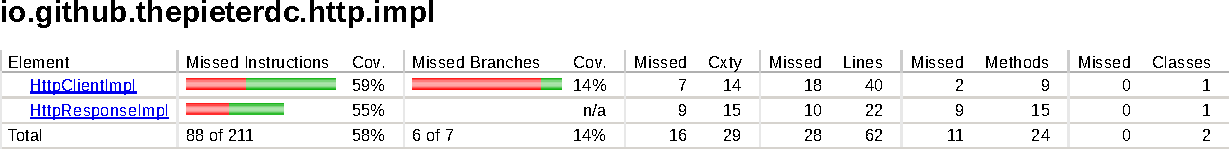
\includegraphics[clip,width=\textwidth]{assets/coverage-jacoco.pdf}
	}
	\newline
	\subfloat[coverage.py report of \url{https://github.com/codecov/example-python}]{%
		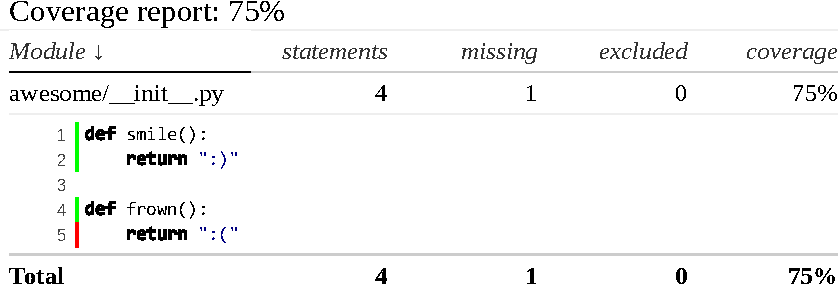
\includegraphics[clip,width=\textwidth]{assets/coverage-coveragepy.pdf}
	}
	\newline
	\subfloat[simplecov report of \url{https://github.com/dodona-edu/dodona}]{%
		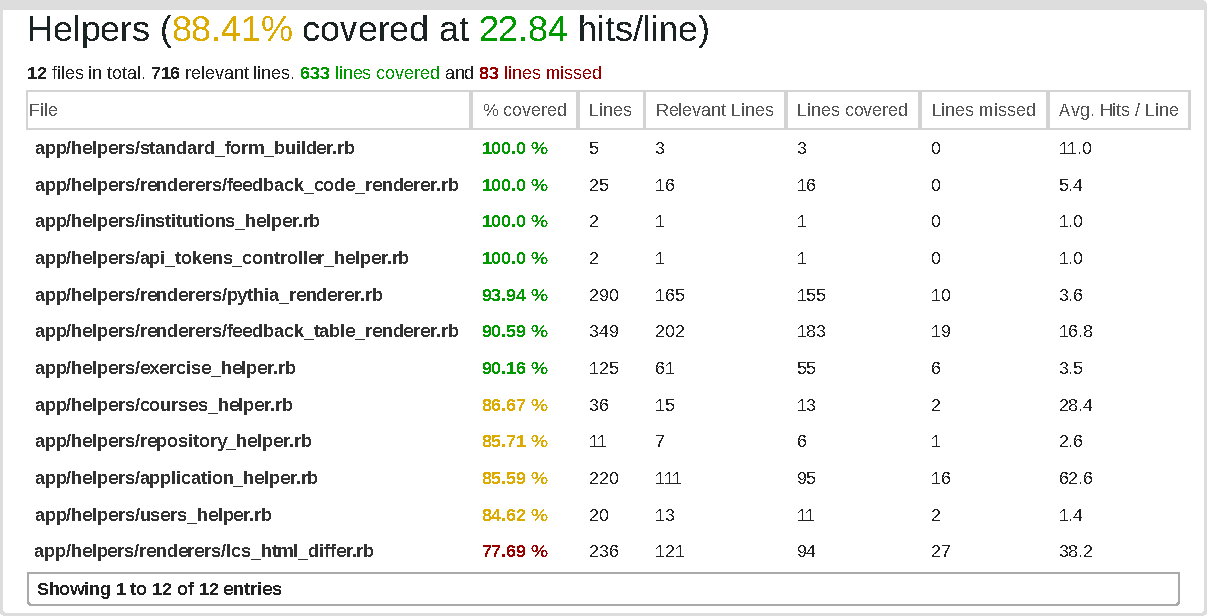
\includegraphics[clip,width=\textwidth]{assets/coverage-simplecov.pdf}
	}
	\caption{Statistics from Code coverage tools}
	\label{fig:coverage-statistics}
\end{figure}